%\documentclass[handout]{beamer}
\documentclass{beamer}
\usepackage{comment}
\usepackage{multirow}
\usepackage{float}
\usepackage{fixltx2e}
\usepackage[boxed]{algorithm2e}
\SetAlFnt{\fontsize{7pt}{8pt}\selectfont \ttfamily}
\SetAlgoInsideSkip{} 
\renewcommand\AlCapFnt{\tiny}
\SetAlCapSkip{1.25ex}
\SetAlgoCaptionLayout{centering}
\setlength{\algomargin}{1.5em}
\SetInd{0.5em}{0.625em}
\usepackage{tikz}
\usepackage{pgfplots}
\usetikzlibrary{shapes.geometric,arrows,fit,matrix,positioning,pgfplots.groupplots}
\tikzset
{
    treenode/.style = {circle, draw=black, align=center, minimum size=1cm},
    subtree/.style  = {isosceles triangle, draw=black, align=center, minimum height=0.25cm, minimum width=0.25cm, shape border rotate=90, anchor=north},
    process/.style={rectangle, minimum width=2cm, minimum height=1cm, align=center, text width=2cm, draw},
    connector/.style={circle, minimum size=1cm, align=center, text width=0.5cm, draw},
    arrow/.style={thick, ->, >=stealth}
}
\usepackage{circuitikz}

\renewcommand\topfraction{0.95}
\renewcommand\bottomfraction{0.95}
\renewcommand\textfraction{0.05} 
\renewcommand\floatpagefraction{0.95}
\renewcommand{\dbltopfraction}{0.95}
\renewcommand{\dblfloatpagefraction}{0.95}	

\floatsep 4pt plus 2pt minus 2pt
\textfloatsep 8pt plus 2pt minus 4pt
\dblfloatsep 4pt plus 2pt minus 2pt
\dbltextfloatsep 8pt plus 2pt minus 4pt

\addtobeamertemplate{navigation symbols}{}{%
    \usebeamerfont{footline}%
    \usebeamercolor[fg]{footline}%
    \hspace{1em}%
    \insertframenumber/\inserttotalframenumber
}
\title{Concurrent Internal Binary Search Trees}
\author[Arun]{\includegraphics[height=0.8cm]{figures/utd_logo.jpg}\\
Arunmoezhi Ramachandran \\
Supervisor - Neeraj Mittal\\
}
\institute[UTDallas]{The University of Texas at Dallas}
\date{}
\begin{document}

\begin{frame}
	\titlepage
\end{frame}

		
\begin{frame}{Overview}
	\tableofcontents
\end{frame}

\section{Introduction}
\begin{frame}{Introduction}
\begin{itemize}
\item \small CPUs aren't getting faster (memory wall, ILP wall and power wall)
\item \small Shift towards multicore and manycore
\end{itemize}
\begin{center}
\Large {\color{red} Problem}\\
How to keep all the cores \textbf{busy}?
\end{center}
\pause
\begin{center}
\Large {\color{blue} Solutions}\\
Parallel computing (obvious choice)\\
\pause
Concurrent computing (a better choice)
\end{center}
\end{frame}

\begin{frame}{Concurrency vs Parallelism}
\begin{center}
\Large {\color{blue}Concurrency} is not {\color{red}parallelism} (it's better!!)
\end{center}
\pause
\begin{columns}
\begin{column}[t]{0.48\textwidth}
\color{red}\rule{\linewidth}{4pt}
Parallel Computing
\setbeamertemplate{itemize/enumerate body begin}{\footnotesize}
\begin{itemize}
\item decades of research done
\item Example - Matrix-Matrix Multiplication
\item \textbf{do} lot of things simultaneously
\item cannot be done on a single CPU
\item \textbf{deterministic} control flow
\item is about \textbf{speedup}
\item \textbf{hard} to debug
\end{itemize}
\end{column}
\begin{column}[t]{0.48\textwidth}
\color{blue}\rule{\linewidth}{4pt}
Concurrent Computing
\setbeamertemplate{itemize/enumerate body begin}{\footnotesize}
\begin{itemize}
\item Relatively new
\item Example - A web crawler, mouse/keyboard
\item \textbf{deal} lot of things simultaneously
\item can be done on a single CPU
\item \textbf{non-deterministic} control flow
\item is about \textbf{hiding latency}
\item \textbf{very hard} to debug
\end{itemize}
\end{column}
\end{columns}
\end{frame}

\section{Design Approaches}
\begin{frame}{Designing Concurrent Data Structures}
\begin{itemize}
\item Shared-memory multiprocessors concurrently execute multiple threads
\item Threads communicate and synchronize through data structures in shared memory
\item Threads can interleave in exponential number of ways
\item Concurrent data structure must preserve its properties for all possible interleavings
\end{itemize}
\end{frame}

\begin{frame}{Example - Shared Counter}
Let $x$ be a shared counter which can be incremented using a function fetchAndIncrement()\\
\pause
Here are some possible implementations of this function\\
\phantom{hello world}
\SetAlgorithmName{fetchAndIncrement}{}{}
\renewcommand{\thealgocf}{}
\begin{minipage}[t]{0.48\textwidth}
\begin{algorithm}[H]
\phantom{acquire(lock)\;}
r1 = x\;
inc(r1)\;
x = r1\;
\phantom{release(lock)\;}

\caption{\tiny sequential}
\end{algorithm}
\pause
\end{minipage}
\begin{minipage}[t]{0.48\textwidth}
\begin{algorithm}[H]
\caption{\tiny Using locks}
acquire(lock)\;
r1 = x\;
inc(r1)\;
x = r1\;
release(lock)\;

\end{algorithm}
\end{minipage}
\pause
\begin{center}
\begin{minipage}[t]{0.65\textwidth}
\begin{algorithm}[H]
\caption{\tiny using atomic instructions}
\Repeat{(x.compareAndSwap(rOld,rNew))}
{
rOld = x\;
rNew = rOld+1\;
}
\end{algorithm}
\end{minipage}
\end{center}
\footnotesize compareAndSwap updates(atomically) the value of $x$ to $rNew$ only if the read value of $x$ is equal to $rOld$. Returns \textit{true} if it succeeds in updating the value of $x$
\end{frame}

\begin{frame}{Design Approaches}
\begin{center}
\Large How to handle contention among threads?
\end{center}
\pause
\begin{itemize}
\item<2-> \Large Blocking Algorithms
\begin{itemize}
\item<3-> use locks to resolve contention
\item<3-> coarse grained or fine grained locking
\item<3->  {\color{black!50!green} easier to design}
\item<3->  {\color{red}weaker progress guarantees} (thread owns a lock) 
\item<3->  {\color{red}are prone to deadlock, priority inversion}
\end{itemize}
\phantom{hello world}
\item<2-> \Large Non-Blocking Algorithms
\begin{itemize}
\item<4->  use atomic (Read-Modify-Write) instructions to resolve contention. E.g. Compare-And-Swap(CAS) instruction
\item<4-> lock-free or wait-free
\item<4-> {\color{black!50!green}stronger progress guarantees} (operation owns a lock - helping)
\item<4-> {\color{black!50!green}deadlock or priority inversion not possible}
\item<4-> {\color{red}harder to design}
\end{itemize}
\end{itemize}
\end{frame}

\section{Binary Search Tree}
\begin{frame}{Binary Search Tree - Defintion}
A \textit{binary search tree} (BST) is a data structure which meets the following requirements:
\begin{itemize}
\item it  is a binary tree (a node can contain atmost two children)
\item each node contains a key $k$
\item left subtree of a node contains keys lesser than $k$
\item right subtree of a node contains keys greater than $k$
\end{itemize}
\pause
Operations on a BST
\begin{itemize}
\item \textbf{search($k$)} - returns \textit{true} only if key $k$ is present in the tree
\item \textbf{insert($k$)} - inserts $k$ into the tree if it does not already exist
\item \textbf{delete($k$)} - deletes $k$ from the tree if it already exist
\end{itemize}
\end{frame}

\begin{frame}{BST - Search}
\textbf{search($70$)}\\
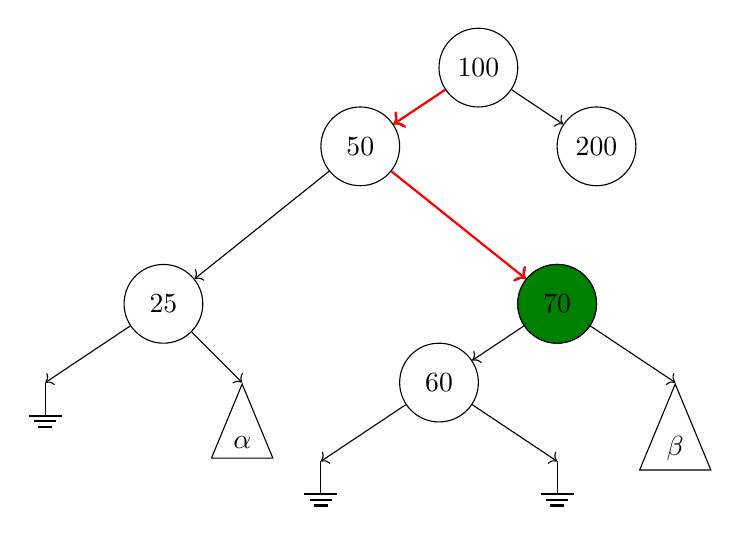
\begin{tikzpicture}
\newcommand\xShift{1.5}
\newcommand\yShift{1}
\node(x) [treenode] at (0, 0) {100};
\node(xl) [treenode] at ([shift=({-\xShift,-\yShift})]x) {50};
\node(xr) [treenode] at ([shift=({\xShift,-\yShift})]x) {200};
\node(xll) [treenode] at ([shift=({-\xShift-1,-\yShift-1})]xl) {25};
\node(xlr) [treenode] at ([shift=({\xShift+1,-\yShift-1})]xl) {70};
\node(xlll) [ground] at ([shift=({-\xShift,-\yShift})]xll) {};
\node(xllr) [subtree] at ([shift=({\xShift-0.5,-\yShift})]xll) {$\alpha$};
\node(xlrl) [treenode] at ([shift=({-\xShift,-\yShift})]xlr) {60};
\node(xlrr) [subtree] at ([shift=({\xShift,-\yShift})]xlr) {$\beta$};
\node(xlrll) [ground] at ([shift=({-\xShift,-\yShift})]xlrl) {};
\node(xlrlr) [ground] at ([shift=({\xShift,-\yShift})]xlrl) {};
\draw[->] (x) -- (xl);
\draw[->] (x) -- (xr);
\draw[->] (xl) -- (xll);
\draw[->] (xl) -- (xlr);
\draw[->] (xll) -- (xlll);
\draw[->] (xll) -- (xllr.north);
\draw[->] (xlr) -- (xlrl);
\draw[->] (xlr) -- (xlrr.north);
\draw[->] (xlrl) -- (xlrll);
\draw[->] (xlrl) -- (xlrlr);
\draw<2->[->,thick,color=red] (x) -- (xl);
\draw<3->[->,thick,color=red] (xl) -- (xlr);
\node<4->(xlr) [treenode,fill=black!50!green] at ([shift=({\xShift+1,-\yShift-1})]xl) {70};
\end{tikzpicture}
\end{frame}

\begin{frame}{BST - Search}
\textbf{search($55$)}\\
\input{figures/BST/searchFalse}
\end{frame}

\begin{frame}{BST - Insert}
\textbf{insert($55$)}\\
\begin{columns}
\begin{column}[t]{0.48\textwidth}
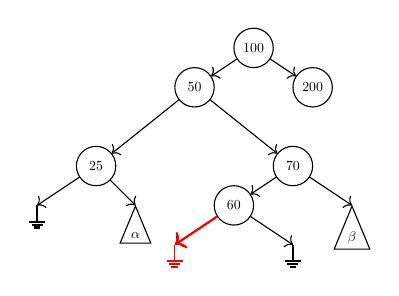
\begin{tikzpicture}[scale=0.5, transform shape]
\newcommand\xShift{1.5}
\newcommand\yShift{1}
\node(x) [treenode] at (0, 0) {100};
\node(xl) [treenode] at ([shift=({-\xShift,-\yShift})]x) {50};
\node(xr) [treenode] at ([shift=({\xShift,-\yShift})]x) {200};
\node(xll) [treenode] at ([shift=({-\xShift-1,-\yShift-1})]xl) {25};
\node(xlr) [treenode] at ([shift=({\xShift+1,-\yShift-1})]xl) {70};
\node(xlll) [ground] at ([shift=({-\xShift,-\yShift})]xll) {};
\node(xllr) [subtree] at ([shift=({\xShift-0.5,-\yShift})]xll) {$\alpha$};
\node(xlrl) [treenode] at ([shift=({-\xShift,-\yShift})]xlr) {60};
\node(xlrr) [subtree] at ([shift=({\xShift,-\yShift})]xlr) {$\beta$};
\node(xlrll) [ground] at ([shift=({-\xShift,-\yShift})]xlrl) {};
\node(xlrlr) [ground] at ([shift=({\xShift,-\yShift})]xlrl) {};
\draw[->] (x) -- (xl);
\draw[->] (x) -- (xr);
\draw[->] (xl) -- (xll);
\draw[->] (xl) -- (xlr);
\draw[->] (xll) -- (xlll);
\draw[->] (xll) -- (xllr.north);
\draw[->] (xlr) -- (xlrl);
\draw[->] (xlr) -- (xlrr.north);
\draw[->] (xlrl) -- (xlrll);
\draw[->] (xlrl) -- (xlrlr);
\draw<2->[->,thick,color=red] (xlrl) -- (xlrll);
\node<2->(xlrll) [ground,color=red] at ([shift=({-\xShift,-\yShift})]xlrl) {};
\end{tikzpicture}
\end{column}
\pause
\pause
\begin{column}[t]{0.5\textwidth}
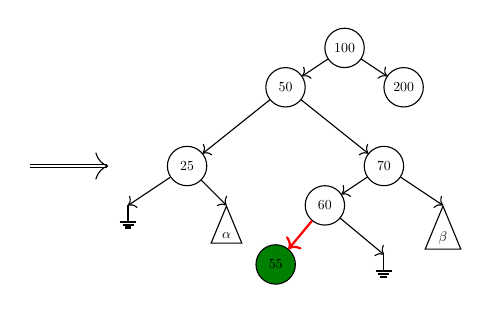
\begin{tikzpicture}[scale=0.5, transform shape]
\draw[->,style=double] (-8,-3) -- (-6,-3){};
\newcommand\xShift{1.5}
\newcommand\yShift{1}
\node(x) [treenode] at (0, 0) {100};
\node(xl) [treenode] at ([shift=({-\xShift,-\yShift})]x) {50};
\node(xr) [treenode] at ([shift=({\xShift,-\yShift})]x) {200};
\node(xll) [treenode] at ([shift=({-\xShift-1,-\yShift-1})]xl) {25};
\node(xlr) [treenode] at ([shift=({\xShift+1,-\yShift-1})]xl) {70};
\node(xlll) [ground] at ([shift=({-\xShift,-\yShift})]xll) {};
\node(xllr) [subtree] at ([shift=({\xShift-0.5,-\yShift})]xll) {$\alpha$};
\node(xlrl) [treenode] at ([shift=({-\xShift,-\yShift})]xlr) {60};
\node(xlrr) [subtree] at ([shift=({\xShift,-\yShift})]xlr) {$\beta$};
\node(xlrll) [treenode,fill=black!50!green] at ([shift=({-\xShift+0.25,-\yShift-0.5})]xlrl) {55};
\node(xlrlr) [ground] at ([shift=({\xShift,-\yShift-0.25})]xlrl) {};
\draw[->] (x) -- (xl);
\draw[->] (x) -- (xr);
\draw[->] (xl) -- (xll);
\draw[->] (xl) -- (xlr);
\draw[->] (xll) -- (xlll);
\draw[->] (xll) -- (xllr.north);
\draw[->] (xlr) -- (xlrl);
\draw[->] (xlr) -- (xlrr.north);
\draw[->,thick,color=red] (xlrl) -- (xlrll);
\draw[->] (xlrl) -- (xlrlr);
\end{tikzpicture}
\end{column}
\end{columns}
\end{frame}

\begin{frame}{Types of delete}
\begin{itemize}
\item simple - removing a node which has atmost one child
\item complex - removing a node which has exactly two children
\end{itemize}
\end{frame}

\begin{frame}{BST - Simple Delete}
\textbf{delete($25$)}
\begin{figure}[b]
\begin{columns}
\begin{column}[t]{0.48\textwidth}
\input{figures/BST/simpleDeleteA}
\end{column}
\pause
\pause
\begin{column}[t]{0.5\textwidth}
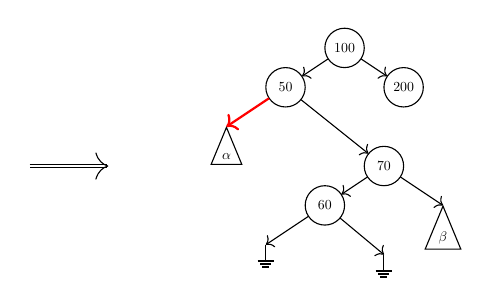
\begin{tikzpicture}[scale=0.5, transform shape]
\draw[->,style=double] (-8,-3) -- (-6,-3){};
\newcommand\xShift{1.5}
\newcommand\yShift{1}
\node(x) [treenode] at (0, 0) {100};
\node(xl) [treenode] at ([shift=({-\xShift,-\yShift})]x) {50};
\node(xr) [treenode] at ([shift=({\xShift,-\yShift})]x) {200};
\node(xll) [subtree] at ([shift=({-\xShift,-\yShift})]xl) {$\alpha$};
\node(xlr) [treenode] at ([shift=({\xShift+1,-\yShift-1})]xl) {70};
\node(xlrl) [treenode] at ([shift=({-\xShift,-\yShift})]xlr) {60};
\node(xlrr) [subtree] at ([shift=({\xShift,-\yShift})]xlr) {$\beta$};
\node(xlrll) [ground] at ([shift=({-\xShift,-\yShift})]xlrl) {};
\node(xlrlr) [ground] at ([shift=({\xShift,-\yShift-0.25})]xlrl) {};
\draw[->] (x) -- (xl);
\draw[->] (x) -- (xr);
\draw[->,thick,color=red] (xl) -- (xll.north);
\draw[->] (xl) -- (xlr);
\draw[->] (xlr) -- (xlrl);
\draw[->] (xlr) -- (xlrr.north);
\draw[->] (xlrl) -- (xlrll);
\draw[->] (xlrl) -- (xlrlr);
\end{tikzpicture}
\end{column}
\end{columns}
\end{figure}
\end{frame}

\begin{frame}{BST - Complex Delete}
\textbf{delete($50$)}
\begin{figure}[b]
\begin{columns}
\begin{column}[t]{0.33\textwidth}
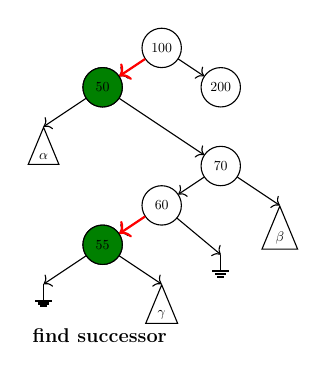
\begin{tikzpicture}[scale=0.5, transform shape]
\newcommand\xShift{1.5}
\newcommand\yShift{1}
\node(x) [treenode] at (0, 0) {100};
\node(xl) [treenode] at ([shift=({-\xShift,-\yShift})]x) {50};
\node(xr) [treenode] at ([shift=({\xShift,-\yShift})]x) {200};
\node(xll) [subtree] at ([shift=({-\xShift,-\yShift})]xl) {$\alpha$};
\node(xlr) [treenode] at ([shift=({\xShift+1.5,-\yShift-1})]xl) {70};
\node(xlrl) [treenode] at ([shift=({-\xShift,-\yShift})]xlr) {60};
\node(xlrr) [subtree] at ([shift=({\xShift,-\yShift})]xlr) {$\beta$};
\node(xlrll) [treenode] at ([shift=({-\xShift,-\yShift})]xlrl) {55};
\node(xlrlr) [ground] at ([shift=({\xShift,-\yShift-0.25})]xlrl) {};
\node(xlrlll) [ground] at ([shift=({-\xShift,-\yShift})]xlrll) {};
\node(xlrllr) [subtree] at ([shift=({\xShift,-\yShift})]xlrll) {$\gamma$};
\draw[->] (x) -- (xl);
\draw[->] (x) -- (xr);
\draw[->] (xl) -- (xll.north);
\draw[->] (xl) -- (xlr);
\draw[->] (xlr) -- (xlrl);
\draw[->] (xlr) -- (xlrr.north);
\draw[->] (xlrl) -- (xlrll);
\draw[->] (xlrl) -- (xlrlr);
\draw[->] (xlrll) -- (xlrlll);
\draw[->] (xlrll) -- (xlrllr.north);
\draw<2->[->,thick,color=red] (x) -- (xl);
\node<2->(xl) [treenode,fill=black!50!green] at ([shift=({-\xShift,-\yShift})]x) {50};
\draw<3->[->,thick,color=red] (xlrl) -- (xlrll);
\node<3->(xlrll) [treenode,fill=black!50!green] at ([shift=({-\xShift,-\yShift})]xlrl) {55};
\node<3->[below right] at (current bounding box.south west) {\Large \textbf{find successor}};
\end{tikzpicture}
\end{column}
\pause
\pause
\pause
\begin{column}[t]{0.33\textwidth}
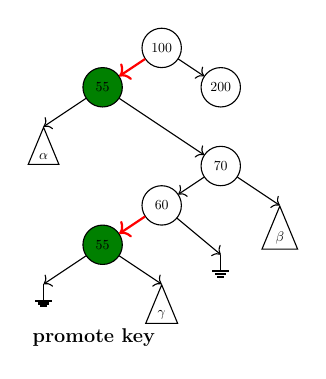
\begin{tikzpicture}[scale=0.5, transform shape]
%\draw[->,style=double] (-8,-3) -- (-7,-3){};
\newcommand\xShift{1.5}
\newcommand\yShift{1}
\node(x) [treenode] at (0, 0) {100};
\node(xl) [treenode,fill=black!50!green] at ([shift=({-\xShift,-\yShift})]x) {55};
\node(xr) [treenode] at ([shift=({\xShift,-\yShift})]x) {200};
\node(xll) [subtree] at ([shift=({-\xShift,-\yShift})]xl) {$\alpha$};
\node(xlr) [treenode] at ([shift=({\xShift+1.5,-\yShift-1})]xl) {70};
\node(xlrl) [treenode] at ([shift=({-\xShift,-\yShift})]xlr) {60};
\node(xlrr) [subtree] at ([shift=({\xShift,-\yShift})]xlr) {$\beta$};
\node(xlrll) [treenode,fill=black!50!green] at ([shift=({-\xShift,-\yShift})]xlrl) {55};
\node(xlrlr) [ground] at ([shift=({\xShift,-\yShift-0.25})]xlrl) {};
\node(xlrlll) [ground] at ([shift=({-\xShift,-\yShift})]xlrll) {};
\node(xlrllr) [subtree] at ([shift=({\xShift,-\yShift})]xlrll) {$\gamma$};
\draw[->,thick,color=red] (x) -- (xl);
\draw[->] (x) -- (xr);
\draw[->] (xl) -- (xll.north);
\draw[->] (xl) -- (xlr);
\draw[->] (xlr) -- (xlrl);
\draw[->] (xlr) -- (xlrr.north);
\draw[->,thick,color=red] (xlrl) -- (xlrll);
\draw[->] (xlrl) -- (xlrlr);
\draw[->] (xlrll) -- (xlrlll);
\draw[->] (xlrll) -- (xlrllr.north);
\node[below right] at (current bounding box.south west) {\Large \textbf{promote key}};
\end{tikzpicture}
\end{column}
\pause
\begin{column}[t]{0.33\textwidth}
\input{figures/BST/complexDeleteC}
\end{column}
\end{columns}
\end{figure}
\end{frame}

\section{Related Works}
\begin{comment}
\begin{frame}{Related Works}
\begin{itemize}
\item lock-free(node-based) external BST by Ellen et.al[PODC'10]
\item lock-free(node-based) internal BST by Howley and Jones[SPAA'12]
\item lock-free(edge-based) external BST by Natarajan and Mittal[PPoPP'14]
\item RCU-based(node-based) internal BST by Arbel and Attiya[PODC'14]
\item lock-based(node-based) internal BST by Drachsler et.al[PPoPP'14]
\end{itemize}
\end{frame}
\end{comment}
\begin{frame}{Related Works}
\begin{table}[h]
\small{
\begin{tabular}{|l|l|c|c|l|}
\hline
\textbf{\#} & \multicolumn{1}{c|}{\textbf{\begin{tabular}[c]{@{}c@{}}Algorithm\\ Type\end{tabular}}} & \textbf{\begin{tabular}[c]{@{}c@{}}Works\\ At\end{tabular}} & \textbf{\begin{tabular}[c]{@{}c@{}}BST\\ Type\end{tabular}} & \multicolumn{1}{c|}{\textbf{Authors}} \\ \hline
1           & lock free                                                                              & node level                                                  & external                                                    & Ellen et.al{[}PODC'10{]}              \\ \hline
2           & lock free                                                                              & node level                                                  & internal                                                    & Howley \& Jones{[}SPAA'12{]}          \\ \hline
3           & lock free                                                                              & edge level                                                  & external                                                    & Natarajan \&Mittal{[}PPoPP'14{]}      \\ \hline
4           & lock based                                                                             & node level                                                  & internal                                                    & Arbel \& Attiya{[}PODC'14{]}          \\ \hline
5           & lock based                                                                             & node level                                                  & internal                                                    & Drachsler et.al{[}PPoPP'14{]}         \\ \hline
\end{tabular}
}
\end{table}
\end{frame}
\section{Lock Based Binary Search Tree}
\begin{frame}[c]{Lock Based BST[PPoPP'15 Poster]}
Contributions
\begin{itemize}
\item combine edge-based locking with internal representation of BST
\item optimistic tree traversal 
\end{itemize}
\end{frame}

\begin{frame}[c]{Lock Based BST[PPoPP'15 Poster]}
\begin{itemize}
\item common workloads have more searches than updates
\begin{itemize}
\item design is optimized for searches
\item search operations are oblivious to locks
\end{itemize}
\pause
\item Any real life workload will have more inserts than deletes
\begin{itemize}
\item insert operations do not obtain any locks
\item performs only one atomic operation
\end{itemize}
\pause
\item removal of a node in a concurrent BST is challenging
\begin{itemize}
\item delete operations uses locks
\item locks can be obtained on nodes or edges
\item locking edges instead of nodes increases concurrency
\end{itemize}
\end{itemize}
\end{frame}

\begin{frame}{Lock Based BST - Challenges in search}
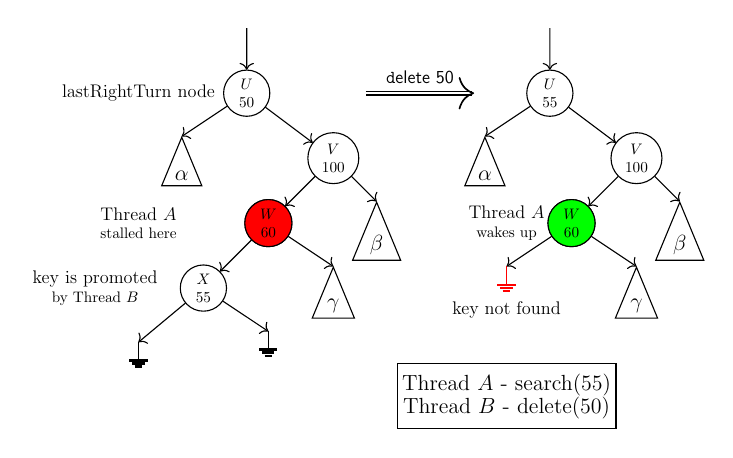
\begin{tikzpicture}[scale=0.55, transform shape,mylabel/.style={thin, draw=black, align=center, minimum width=0.3cm, minimum height=0.3cm,fill=white}]
		\newcommand\XA{0}
		\newcommand\YA{0}
		\node (x)		[treenode] 									at (-6,0)       							{$U$ \\ 50};
		\node (a)		[subtree] 									at (-7.5,-1)  								{\Large $\alpha$};
		\node (y0)	[treenode] 									at (-4,-1.5) 									{$V$ \\ 100};
		\node (y1)	[treenode]									at (-5.5,-3)									{$W$ \\ 60}; 
		\node (b)		[subtree] 									at (-3,-2.5)    							{\Large $\beta$};
		\node (y2)	[treenode]									at (-7,-4.5)									{$X$ \\ 55}; 
		\node (g)		[subtree] 									at (-4,-4)   									{\Large $\gamma$};
		\node (gnd)	[ground] 										at (-8.5,-5.75)								{}; 
		\node (o)		[ground] 										at (-5.5,-5.5)  							{};
		\node (x1) 	[] 													at (-8.5,0) 									{\large lastRightTurn node};
		\draw[->] (-6, 1.5) --  (x);
		\draw[->] (x) -- (y0);
		\draw[->] (x) -- (a.north);
		\draw[->] (y0) -- (y1);
		\draw[->] (y0) -- (b.north);
		\draw[->] (y1) -- (y2);
		\draw[->] (y1) -- (g.north);
		\draw[->] (y2) -- (gnd);
		\draw[->] (y2) -- (o);
		%% legend
		\node [thin, draw=black, align=center, minimum width=5cm, minimum height=1.5cm] at (0,-7) {\Large Thread $A$ - search(55) \\ \Large Thread $B$ - delete(50)};	
		\pause
		\node (y1)	[treenode, fill=red]		at (-5.5,-3)											{$W$ \\ 60}; 
		\node (y1l) [rectangle,align=center,minimum size=1cm] at (-8.5,-3) 		{\large Thread $A$ \\stalled here};
		\pause
		\node (y2l) [rectangle,align=center,minimum size=1cm] at(-9.5,-4.5) 	{\large key is promoted \\by Thread $B$};
		\pause
		\path[every node/.style={font=\sffamily\small}]
		(-3.25, 0) edge[->,semithick, double] node [above, outer sep=3pt] 		{\large \texttt delete 50} (-0.75, 0);

		\node (ix)	[treenode] 									at (1,0)       								{$U$ \\ 55};
		\node (ia)	[subtree] 									at (-0.5,-1)  								{\Large $\alpha$};
		\node (iy0)	[treenode] 									at (3,-1.5) 									{$V$ \\ 100};
		\node (iy1)	[treenode, fill=red]									at (1.5,-3)					{$W$ \\ 60}; 
		\node (ib)	[subtree] 									at (4,-2.5)    								{\Large $\beta$};
		\node (io)	[ground]										at (0,-4)											{}; 
		\node (ignd)[subtree] 									at (3,-4)   									{\Large $\gamma$};
    
    \draw[->] (1, 1.5) --  (ix);
    \draw[->] (ix) --  (iy0);
    \draw[->] (ix) --  (ia.north);
    \draw[->] (iy0) --  (iy1);
    \draw[->] (iy0) --  (ib.north);
    \draw[->] (iy1) --  (io);
    \draw[->] (iy1) --  (ignd.north);
		\pause
		\node (iy1)	[treenode, fill=green]									at (1.5,-3)					{$W$ \\ 60};
		\node (y12) [rectangle,align=center,minimum size=1cm] at (0,-3) 		{\large Thread $A$ \\wakes up};
		\pause
		\node (io)	[ground,color=red]										at (0,-4)											{}; 
		\node (y13) [rectangle,align=center,minimum size=1cm] at (0,-5) 		{\large key not found};
	\end{tikzpicture}
\visible<6>
{
\\Keep track of last right turn node and its key. If search terminates at a NULL node, check if the current key in the last right turn node has changed. If yes restart the operation from root.
}
\end{frame}

\begin{frame}[c]{Lock Based BST - Delete}
pseudocode for delete
\begin{algorithm}[H]
locate the node to delete\;
\uIf{simple delete}
{
lock the edge $\langle$parent,node$\rangle$\;
lock the children edges\;
make the parent point to the non-null child using a simple write instruction\;
release all locks\;
}
\Else(// complex delete)
{
lock the edge $\langle$node,rightChild$\rangle$\;
find the successor\;
lock the edge $\langle$successorParent,successor$\rangle$\;
lock the children edges of successor\;
promote key\;
remove successor by a making successorParent point to non-null child of successor\;
release all locks\;
}
\end{algorithm}
\end{frame}

\begin{frame}[c]{Lock Based BST - Simple Delete}
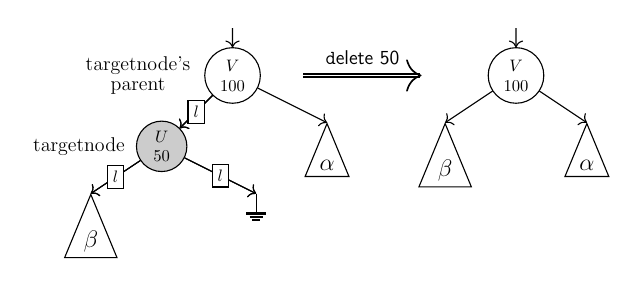
\begin{tikzpicture}[scale=0.6, transform shape,mylabel/.style={thin, draw=black, align=center, minimum width=0.3cm, minimum height=0.3cm,fill=white}]
		\newcommand\XA{-3}
		\newcommand\YA{0}
		\node (x)		[treenode] 																at (\XA,\YA)       					{$V$ \\ 100};
		\node (y)		[treenode, fill=black!20] 								at (\XA-1.5,\YA-1.5) 				{$U$ \\ 50};
		\node (a)		[subtree] 																at (\XA+2,\YA-1)      			{\Large $\alpha$};
		\node (b)		[subtree] 																at (\XA-3,\YA-2.5)    			{\Large $\beta$};
		\node (gnd)	[ground] 																	at (\XA+0.5,\YA-2.5)				{}; 
		\node (xl) 	[rectangle,align=center,minimum size=1cm] at (\XA-2,\YA) 							{\large targetnode's \\ \large parent};
		\node (yl) 	[] 																				at (\XA-3.25,\YA-1.5) 			{\large targetnode};
		
 		\draw[->] (x) -- (y);
 		\draw[->] (y) -- (b.north);
 		\draw[->] (y) -- (gnd);
		\draw[->] (\XA,\YA+1) -- (x);
		\draw[->] (x) -- (a.north);
		\pause
		\draw[->] (x) -- node[mylabel] {$\boldsymbol{l}$} (y);
		\pause
		\draw[->] (y) -- node[mylabel] {$\boldsymbol{l}$} (b.north);
		\pause
		\draw[->] (y) -- node[mylabel] {$\boldsymbol{l}$} (gnd);
    \pause
		\path[every node/.style={font=\sffamily\small}]
		(\XA+1.5,\YA) edge[->,semithick, double] 							node [above, outer sep=3pt] {\large \texttt delete 50} (\XA+4,\YA);
		
		\node (ix)	[treenode] 																at (\XA+6,\YA) 							{$V$ \\ 100};
		\node (ib)	[subtree] 																at (\XA+4.5,\YA-1)					{\Large $\beta$};
		\node (ia)	[subtree] 																at (\XA+7.5,\YA-1) 					{\Large $\alpha$};

		\draw[->] (\XA+6,\YA+1) -- (ix);
		\draw[->] (ix) -- (ib.north);
		\draw[->] (ix) -- (ia.north);
	\end{tikzpicture}
\end{frame}

\begin{frame}[c]{Lock Based BST - Complex Delete}
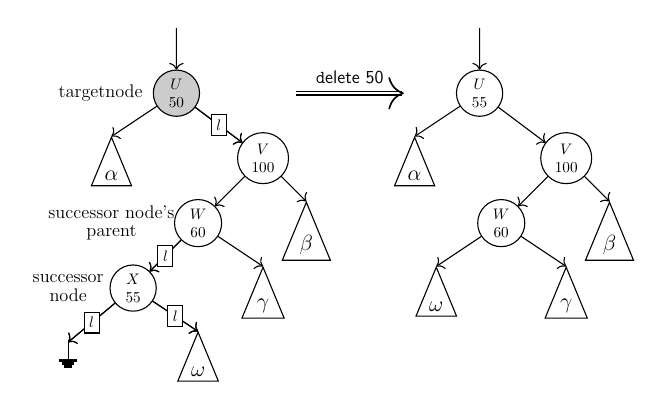
\begin{tikzpicture}[scale=0.55, transform shape,mylabel/.style={thin, draw=black, align=center, minimum width=0.3cm, minimum height=0.3cm,fill=white}]
		\newcommand\XA{0}
		\newcommand\YA{0}
		\node (x)		[treenode, fill=black!20] 	at (-6,0)       							{$U$ \\ 50};
		\node (a)		[subtree] 									at (-7.5,-1)  								{\Large $\alpha$};
		\node (y0)	[treenode] 									at (-4,-1.5) 									{$V$ \\ 100};
		\node (y1)	[treenode]									at (-5.5,-3)									{$W$ \\ 60}; 
		\node (b)		[subtree] 									at (-3,-2.5)    							{\Large $\beta$};
		\node (y2)	[treenode]									at (-7,-4.5)									{$X$ \\ 55}; 
		\node (g)		[subtree] 									at (-4,-4)   									{\Large $\gamma$};
		\node (gnd)	[ground] 										at (-8.5,-5.75)									{}; 
		\node (o)		[subtree] 									at (-5.5,-5.5)  							{\Large $\omega$};
		\node (x1) 	[] 													at (-7.75,0) 									{\large targetnode};
		\node (y1l) [rectangle,align=center,minimum size=1cm] at (-7.5,-3) 		{\large successor node's \\ \large parent};
		\node (y2l) [rectangle,align=center,minimum size=1cm] at(-8.5,-4.5) 	{\large successor \\ \large node};
		
		\draw[->] (-6, 1.5) --  (x);
		\draw[->] (x) -- (y0);
		\draw[->] (x) -- (a.north);
		\draw[->] (y0) -- (y1);
		\draw[->] (y0) -- (b.north);
		\draw[->] (y1) -- (y2);
		\draw[->] (y1) -- (g.north);
		\draw[->] (y2) -- (gnd);
		\draw[->] (y2) -- (o.north);
    \pause
    \draw[->] (x) -- node[mylabel] {$\boldsymbol{l}$} (y0);
    \pause
    \draw[->] (y1) -- node[mylabel] {$\boldsymbol{l}$} (y2);
    \pause
    \draw[->] (y2) -- node[mylabel] {$\boldsymbol{l}$} (gnd);
    \pause
  	\draw[->] (y2) -- node[mylabel] {$\boldsymbol{l}$} (o.north);
    \pause
		\path[every node/.style={font=\sffamily\small}]
		(-3.25, 0) edge[->,semithick, double] node [above, outer sep=3pt] 		{\large \texttt delete 50} (-0.75, 0);

		\node (ix)	[treenode] 									at (1,0)       								{$U$ \\ 55};
		\node (ia)	[subtree] 									at (-0.5,-1)  								{\Large $\alpha$};
		\node (iy0)	[treenode] 									at (3,-1.5) 									{$V$ \\ 100};
		\node (iy1)	[treenode]									at (1.5,-3)										{$W$ \\ 60}; 
		\node (ib)	[subtree] 									at (4,-2.5)    								{\Large $\beta$};
		\node (io)	[subtree]										at (0,-4)											{\Large $\omega$}; 
		\node (ignd)[subtree] 									at (3,-4)   									{\Large $\gamma$};
    
    \draw[->] (1, 1.5) --  (ix);
    \draw[->] (ix) --  (iy0);
    \draw[->] (ix) --  (ia.north);
    \draw[->] (iy0) --  (iy1);
    \draw[->] (iy0) --  (ib.north);
    \draw[->] (iy1) --  (io.north);
    \draw[->] (iy1) --  (ignd.north);
	\end{tikzpicture}
\end{frame}

\begin{frame}{Lock Based BST - More challenges in search}
A scenario in which the last right turn node is removed
\begin{figure}
\centering
{
	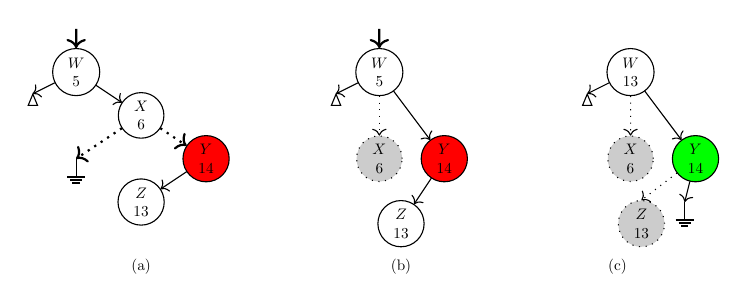
\begin{tikzpicture}[scale=0.55, transform shape]
		\newcommand\XA{-7}
		\newcommand\YA{0}
		\node[] at (-5.5,-4.5) {(a)};
		\node (x)		[treenode] 									at (\XA,\YA)       						{$W$ \\ 5};
		\node (S1)	[subtree,scale=0.5] 				at ([shift=({-1,-0.5})]x)  		{};
		\node (y0)	[treenode] 									at ([shift=({1.5,-1})]x) 			{$X$ \\ 6};
		\node (gnd)	[ground]										at ([shift=({-1.5,-1})]y0)		{}; 
		\node (y1)	[treenode,fill=red] 				at ([shift=({1.5,-1})]y0)   	{$Y$ \\ 14};
		\node (y2)	[treenode] 									at ([shift=({-1.5,-1})]y1)  	{$Z$ \\ 13};
		%\node (S2)	[subtree,scale=0.5]					at ([shift=({0.5,-1})]y1)			{}; 

		\path[every node/.style={font=\sffamily\large}]
		(\XA,\YA+1) 	edge[->,thick] 		node 					{} (x)
		(x) 		edge[->]								node 					{} (S1.north)
		(x) 		edge[->]								node 					{} (y0)
		(y0) 		edge[->,dotted,thick]		node 					{} (gnd)
		(y0) 		edge[->,dotted,thick]		node 					{} (y1)
		(y1) 		edge[->]								node 					{} (y2);
		%(y1) 		edge[->]							node 					{} (S2.north);
		\pause
		\renewcommand\XA{0}
		\node[] at (0.5,-4.5) {(b)};
		\node (ix)	[treenode] 										at (\XA,\YA)       						{$W$ \\ 5};
		\node (iS1)	[subtree,scale=0.5] 					at ([shift=({-1,-0.5})]ix)  	{};
		\node (iy1)	[treenode,fill=red] 					at ([shift=({1.5,-2})]ix)   {$Y$ \\ 14};
		\node (iy2)	[treenode] 										at ([shift=({-1,-1.5})]iy1)  	{$Z$ \\ 13};
		%\node (iS2)	[subtree,scale=0.5]					at ([shift=({0.5,-1.0})]iy1)	{}; 
		\node (iy0)	[treenode, fill=black!20, dotted] at ([shift=({0,-2})]ix) {$X$ \\ 6};

		\path[every node/.style={font=\sffamily\large}]
		(\XA,\YA+1) 	edge[->,thick] 		node 					{} (ix)
		(ix) 		edge[->]								node 					{} (iS1.north)
		(ix) 		edge[->]								node 					{} (iy1)
		(ix) 		edge[->,dotted]					node 					{} (iy0)
		(iy1) 	edge[->]								node 					{} (iy2);
		%(iy1) 	edge[->]								node 					{} (iS2.north);
		\pause
		\renewcommand\XA{5.8}
		\node[] at (5.5,-4.5) {(c)};
		\node (iix)		[treenode] 									at (\XA,\YA)       							{$W$ \\ 13};
		\node (iiS1)	[subtree,scale=0.5] 				at ([shift=({-1,-0.5})]iix)  		{};
		\node (iiy1)	[treenode,fill=green] 			at ([shift=({1.5,-2})]iix)  		{$Y$ \\ 14};
		\node (iignd)	[ground]										at ([shift=({-0.25,-1})]iiy1)				{}; 
		\node (iy0)	[treenode, fill=black!20, dotted] at ([shift=({0,-2})]iix) {$X$ \\ 6};
		\node (iy2)	[treenode, fill=black!20, dotted] at ([shift=({-1.25,-1.5})]iiy1){$Z$ \\ 13};
		
		\path[every node/.style={font=\sffamily\large}]
		(iix) 		edge[->]								node 					{} (iiS1.north)
		(iix) 		edge[->]								node 					{} (iiy1)
		(iix) 		edge[->,dotted]					node 					{} (iy0)
		(iiy1) 		edge[->,dotted]					node 					{} (iy2.north)
		(iiy1) 		edge[->]								node 					{} (iignd);	
	\end{tikzpicture}
}
\end{figure}

\begin{itemize}
\item<1> \footnotesize Search(13) gets stalled at $Y$ in (a). Its last right turn node is $X$
\item<2> \footnotesize Delete(6) removes $X$ from the tree in (b). The key stored in $X$ is still 6
\item<3> \footnotesize Delete(5) results in 13 moving up the tree from $Z$ to $W$ in (c). When search(13) wakes up, it will miss 13 as the key in the last right turn node has not changed
\end{itemize}


\begin{itemize}
\item<4> \footnotesize In the first traversal search(13) saw the node $X$
\item<4> \footnotesize In the second traversal there are two cases
\begin{itemize}
\item<4> \tiny case1, search(13) did not find $X$ - save the traversal and restart
\item<4> \tiny case2, search(13) did find $X$ - use the results of previous traversal
\end{itemize}
\end{itemize}

\end{frame}

\section{Lock Free Binary Search Tree}
\begin{frame}[c]{Lock Free BST[ICDCN'15]}
Contributions
\begin{itemize}
\item combine edge-based locking with internal representation of BST 
\item optimistic tree traversal 
\pause
\item lock-free algorithm
\end{itemize}
\end{frame}

\begin{frame}{Lock Free BST[ICDCN'15]}
\begin{itemize}
\item search and inserts are same as in lock Based BST
\item to maintain lock-free property, if an insert or delete operation fails, it helps a pending delete operation(if needed)
\end{itemize} 
pseudocode for delete
\begin{algorithm}[H]
locate the node to delete\;
flag the children edges for deletion\;
\uIf{simple delete}
{
make the parent point to the non-null child atomically\;
}
\Else(// complex delete)
{
find the successor\;
flag the children edges of successor for promotion\;
promote key\;
remove successor by a simple delete\;
replace node with a fresh copy\;
}
\end{algorithm}
\end{frame}

\begin{frame}[c]{Lock Free BST - Simple Delete}
\begin{itemize}
\item flag is owned by an operation
\item if a thread which installed the flag is stalled, other threads can help complete the operation
\end{itemize}
\pause
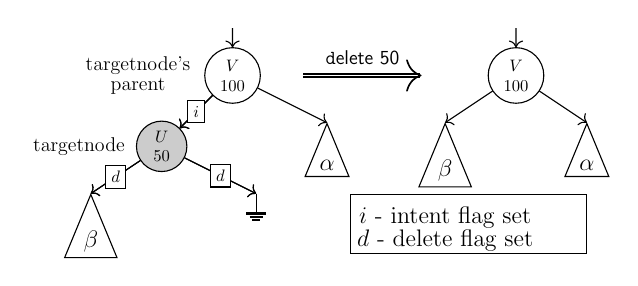
\begin{tikzpicture}[scale=0.6, transform shape,mylabel/.style={thin, draw=black, align=center, minimum width=0.3cm, minimum height=0.3cm,fill=white}]
		\newcommand\XA{-3}
		\newcommand\YA{0}
		\node (x)		[treenode] 																at (\XA,\YA)       					{$V$ \\ 100};
		\node (y)		[treenode, fill=black!20] 								at (\XA-1.5,\YA-1.5) 				{$U$ \\ 50};
		\node (a)		[subtree] 																at (\XA+2,\YA-1)      			{\Large $\alpha$};
		\node (b)		[subtree] 																at (\XA-3,\YA-2.5)    			{\Large $\beta$};
		\node (gnd)	[ground] 																	at (\XA+0.5,\YA-2.5)				{}; 
		\node (xl) 	[rectangle,align=center,minimum size=1cm] at (\XA-2,\YA) 							{\large targetnode's \\ \large parent};
		\node (yl) 	[] 																				at (\XA-3.25,\YA-1.5) 			{\large targetnode};
		
 		\draw[->] (x) -- (y);
 		\draw[->] (y) -- (b.north);
 		\draw[->] (y) -- (gnd);
		\draw[->] (\XA,\YA+1) -- (x);
		\draw[->] (x) -- (a.north);
		\pause
		%% legend
		\node (l1) 																						at (\XA+4.5,\YA-3){\Large $\boldsymbol{i}$  - \Large intent flag set};
		\node (l2) 																						at (\XA+4.5,\YA-3.5){\Large $\boldsymbol{d}$  - \Large delete flag set};
		\node [thin, draw=black, align=center, minimum width=5cm, minimum height=1.25cm] at (\XA+5,\YA-3.15) {};	
		\draw[->] (x) -- node[mylabel] {$\boldsymbol{i}$} (y);
		%\draw[->] (x) -- node[mylabel] {$\boldsymbol{f}$} (y);
		\pause
		\draw[->] (y) -- node[mylabel] {$\boldsymbol{d}$} (b.north);
		%\draw[->] (y) -- node[mylabel] {$\boldsymbol{f}$} (b.north);
		\pause
		\draw[->] (y) -- node[mylabel] {$\boldsymbol{d}$} (gnd);
		%\draw[->] (y) -- node[mylabel] {$\boldsymbol{f}$} (gnd);
    \pause
		\path[every node/.style={font=\sffamily\small}]
		(\XA+1.5,\YA) edge[->,semithick, double] 							node [above, outer sep=3pt] {\large \texttt delete 50} (\XA+4,\YA);
		
		\node (ix)	[treenode] 																at (\XA+6,\YA) 							{$V$ \\ 100};
		\node (ib)	[subtree] 																at (\XA+4.5,\YA-1)					{\Large $\beta$};
		\node (ia)	[subtree] 																at (\XA+7.5,\YA-1) 					{\Large $\alpha$};

		\draw[->] (\XA+6,\YA+1) -- (ix);
		\draw[->] (ix) -- (ib.north);
		\draw[->] (ix) -- (ia.north);
	\end{tikzpicture}
\end{frame}

\begin{frame}[c]{Lock Free BST - Complex Delete}
\input{figures/ICDCNcomplexDelete1}
\end{frame}
\begin{frame}[c]{Lock Free BST - Complex Delete}
\input{figures/ICDCNcomplexDelete2}
\end{frame}

\section{Experimental Evaluation}
\begin{frame}{Experimental Setup}
To compare the performance of various concurrent BSTs we considered the following parameters:
\begin{itemize}
\item Maximum Tree Size
  \begin{itemize}
  \item key space size varied from 2\textsuperscript{13} (8Ki) to 2\textsuperscript{24} (16Mi).
  \end{itemize}
\item Relative Distribution of Operations
  \begin{itemize}
  \item Read-Dominated\phantom{1}(90\% search, \phantom{1}9\% insert and \phantom{1}1\% delete)
  \item Mixed\phantom{1234567890}(70\% search, 20\% insert and 10\% delete)
  \item Write-Dominated (\phantom{1}0\% search, 50\% insert and 50\% delete)
  \end{itemize}
\item Maximum degree of Contention
  \begin{itemize}
  \item number of threads that can concurrently operate on the tree
  \item we collected data for 32 threads
  \end{itemize}
\end{itemize}
\end{frame}

\begin{frame}{Experimental Setup}
\small
{
\begin{itemize}
\item Throughput computed as millions of operations per second (MOPS)
\item each trial was run for 10 seconds
\item Average over 3 trials
\item \textit{pre-populated} the tree to 50\% of its maximum size to capture steady state behaviour
\item beginning of each run consisted of a ``warm-up'' phase whose numbers were excluded in the computed statistics to avoid initial caching effects
\item The machine we used is a Dell PowerEdge R820 server with 4 Intel E5-4650 @ 2.70GHz 8-core processors (32 cores in total) and 1TB of DDR3 memory with HT disabled. 256KB L2 and 20MB shared L3
\end{itemize}
}
\end{frame}

\begin{frame}{Other Concurrent BSTs}
\begin{itemize}
\item a lock-free internal BST by Howley and Jones[SPAA'12], denoted by HJ-BST
\item a lock-free external BST by Natarajan and Mittal[PPoPP'14], denoted by NM-BST
\item RCU-based internal BST by Arbel and Attiya[PODC'14], denoted by CITRUS 
\end{itemize}
\end{frame}

\begin{frame}{Lock Based BST}
% Style to select only points from #1 to #2 (inclusive)
\pgfplotsset
{
	select coords between index/.style 2 args=
	{
    x filter/.code=
		{
        \ifnum\coordindex<#1\def\pgfmathresult{}\fi
        \ifnum\coordindex>#2\def\pgfmathresult{}\fi
    }
	}
}
\begin{figure}[h]
\centering
\begin{tikzpicture}[scale=0.9, transform shape]
		\begin{groupplot}[group style={group size= 3 by 3,vertical sep=0.75cm},height=3cm,width=4cm,xmode=log,log basis x={2},max space between ticks=20,minor tick num=1,tick label style={font=\tiny},xlabel style={font=\tiny},ylabel style={font=\tiny}, title style={font=\tiny}]
		\nextgroupplot[title=Small,ylabel={Read-Dominated},xtick=data]
				\addplot[red,semithick,mark=triangle] 	[select coords between index={3}{6}] table{Data/HJ-BST.dat};  \label{plots:HJ-BST:1}
				\addplot[blue,semithick,mark=asterisk] 	[select coords between index={3}{6}] table{Data/NM-BST.dat};  \label{plots:NM-BST:2}
				\addplot[brown, semithick,mark=square] 	[select coords between index={3}{6}] table{Data/CITRUS.dat};  \label{plots:CITRUS:3}
				\addplot[green, semithick,mark=o] 			[select coords between index={3}{6}] table{Data/RM-LOCK.dat};  \label{plots:RM-LOCK:4}
				\coordinate (top) at (rel axis cs:0,1);% coordinate at top of the first plot
		\nextgroupplot[title=Medium,xtick=data] 
				\addplot[red,semithick,mark=triangle] 	[select coords between index={7}{10}] table{Data/HJ-BST.dat};
				\addplot[blue,semithick,mark=asterisk] 	[select coords between index={7}{10}] table{Data/NM-BST.dat};
				\addplot[brown, semithick,mark=square] 	[select coords between index={7}{10}] table{Data/CITRUS.dat};
				\addplot[green, semithick,mark=o] 			[select coords between index={7}{10}] table{Data/RM-LOCK.dat}; 
		\nextgroupplot[title=Large,xtick=data]
				\addplot[red,semithick,mark=triangle] 	[select coords between index={11}{14}] table{Data/HJ-BST.dat};
				\addplot[blue,semithick,mark=asterisk] 	[select coords between index={11}{14}] table{Data/NM-BST.dat};
				\addplot[brown, semithick,mark=square] 	[select coords between index={11}{14}] table{Data/CITRUS.dat};
				\addplot[green, semithick,mark=o] 			[select coords between index={11}{14}] table{Data/RM-LOCK.dat};
		\nextgroupplot[ylabel={Mixed},xtick=data]
				\addplot[red,semithick,mark=triangle] 	[select coords between index={18}{21}] table{Data/HJ-BST.dat};
				\addplot[blue,semithick,mark=asterisk] 	[select coords between index={18}{21}] table{Data/NM-BST.dat};
				\addplot[brown, semithick,mark=square] 	[select coords between index={18}{21}] table{Data/CITRUS.dat};
				\addplot[green, semithick,mark=o] 			[select coords between index={18}{21}] table{Data/RM-LOCK.dat};
		\nextgroupplot[xtick=data]
				\addplot[red,semithick,mark=triangle] 	[select coords between index={22}{25}] table{Data/HJ-BST.dat};
				\addplot[blue,semithick,mark=asterisk] 	[select coords between index={22}{25}] table{Data/NM-BST.dat};
				\addplot[brown, semithick,mark=square] 	[select coords between index={22}{25}] table{Data/CITRUS.dat};
				\addplot[green, semithick,mark=o] 			[select coords between index={22}{25}] table{Data/RM-LOCK.dat};
		\nextgroupplot[xtick=data]
				\addplot[red,semithick,mark=triangle] 	[select coords between index={26}{29}] table{Data/HJ-BST.dat};
				\addplot[blue,semithick,mark=asterisk] 	[select coords between index={26}{29}] table{Data/NM-BST.dat};
				\addplot[brown, semithick,mark=square] 	[select coords between index={26}{29}] table{Data/CITRUS.dat};
				\addplot[green, semithick,mark=o] 			[select coords between index={26}{29}] table{Data/RM-LOCK.dat};
		\nextgroupplot[xlabel={Key Space Size},ylabel={Write-Dominated},xtick=data]
				\addplot[red,semithick,mark=triangle] 	[select coords between index={33}{36}] table{Data/HJ-BST.dat};
				\addplot[blue,semithick,mark=asterisk] 	[select coords between index={33}{36}] table{Data/NM-BST.dat};
				\addplot[brown, semithick,mark=square] 	[select coords between index={33}{36}] table{Data/CITRUS.dat};
				\addplot[green, semithick,mark=o] 			[select coords between index={33}{36}] table{Data/RM-LOCK.dat};
		\nextgroupplot[xlabel={Key Space Size},xtick=data]
				\addplot[red,semithick,mark=triangle] 	[select coords between index={37}{40}] table{Data/HJ-BST.dat};
				\addplot[blue,semithick,mark=asterisk] 	[select coords between index={37}{40}] table{Data/NM-BST.dat};
				\addplot[brown, semithick,mark=square] 	[select coords between index={37}{40}] table{Data/CITRUS.dat};
				\addplot[green, semithick,mark=o] 			[select coords between index={37}{40}] table{Data/RM-LOCK.dat};
		\nextgroupplot[xlabel={Key Space Size},xtick=data]
				\addplot[red,semithick,mark=triangle] 	[select coords between index={41}{44}] table{Data/HJ-BST.dat};
				\addplot[blue,semithick,mark=asterisk] 	[select coords between index={41}{44}] table{Data/NM-BST.dat};
				\addplot[brown, semithick,mark=square] 	[select coords between index={41}{44}] table{Data/CITRUS.dat};
				\addplot[green, semithick,mark=o] 			[select coords between index={41}{44}] table{Data/RM-LOCK.dat};						
				\coordinate (bot) at (rel axis cs:1,0);% coordinate at bottom of the last plot
	\end{groupplot}
	\path (top-|current bounding box.west)-- node[anchor=south,rotate=90] {\tiny Relative throughput (million operations/second)} (bot-|current bounding box.west);
	\path (top|-current bounding box.north)-- coordinate(legendpos) (bot|-current bounding box.north);
	\matrix[matrix of nodes, anchor=south, draw, inner sep=0.2em, draw] at ([yshift=1ex]legendpos)
  {
    \ref{plots:HJ-BST:1}& \tiny HJ-BST & [3pt]
    \ref{plots:NM-BST:2}& \tiny NM-BST & [3pt]
    \ref{plots:CITRUS:3}& \tiny CITRUS & [3pt]
		\ref{plots:RM-LOCK:4}& \tiny CASTLE \\
	};
\end{tikzpicture}
\end{figure}
\end{frame}

\begin{frame}{Lock Free BST}
% Style to select only points from #1 to #2 (inclusive)
\pgfplotsset
{
	select coords between index/.style 2 args=
	{
    x filter/.code=
		{
        \ifnum\coordindex<#1\def\pgfmathresult{}\fi
        \ifnum\coordindex>#2\def\pgfmathresult{}\fi
    }
	}
}
\begin{figure}[h]
\centering
%% \large
\begin{tikzpicture}[scale=0.9, transform shape]
	\begin{groupplot}[group style={group size= 3 by 3,vertical sep=0.75cm},height=3cm,width=4cm,xmode=log,log basis x={2},max space between ticks=20,minor tick num=1,tick label style={font=\tiny},xlabel style={font=\tiny},ylabel style={font=\tiny}, title style={font=\tiny}]
		\nextgroupplot[title=small,ylabel={Read-Dominated},xtick=data]
				\addplot[red,semithick,mark=triangle] 	[select coords between index={3}{6}] table[x=keyspace, y=MOPS, col sep=tab] {Data/HJ-BST-Keysweep.csv};  \label{plots:HJ-BST-K}
				\addplot[blue,semithick,mark=asterisk]  [select coords between index={3}{6}] table[x=keyspace, y=MOPS, col sep=tab] {Data/NM-BST-Keysweep.csv};  \label{plots:NM-BST-K}
				\addplot[brown, semithick,mark=square]  [select coords between index={3}{6}] table[x=keyspace, y=MOPS, col sep=tab] {Data/CITRUS-Keysweep.csv};  \label{plots:CITRUS-K}
				\addplot[green, semithick,mark=o] 			[select coords between index={3}{6}] table[x=keyspace, y=MOPS, col sep=tab] {Data/RM-BST-Keysweep.csv};  \label{plots:RM-BST-K}
				\coordinate (top) at (rel axis cs:0,1);% coordinate at top of the first plot
		\nextgroupplot[title=Medium,xtick=data]
				\addplot[red,semithick,mark=triangle] 	[select coords between index={7}{10}] table[x=keyspace, y=MOPS, col sep=tab] {Data/HJ-BST-Keysweep.csv};
				\addplot[blue,semithick,mark=asterisk] 	[select coords between index={7}{10}] table[x=keyspace, y=MOPS, col sep=tab] {Data/NM-BST-Keysweep.csv};
				\addplot[brown, semithick,mark=square]  [select coords between index={7}{10}] table[x=keyspace, y=MOPS, col sep=tab] {Data/CITRUS-Keysweep.csv};
				\addplot[green, semithick,mark=o] 			[select coords between index={7}{10}] table[x=keyspace, y=MOPS, col sep=tab] {Data/RM-BST-Keysweep.csv};
		\nextgroupplot[title=Large,xtick=data]
				\addplot[red,semithick,mark=triangle] 	[select coords between index={11}{14}] table[x=keyspace, y=MOPS, col sep=tab] {Data/HJ-BST-Keysweep.csv};
				\addplot[blue,semithick,mark=asterisk] 	[select coords between index={11}{14}] table[x=keyspace, y=MOPS, col sep=tab] {Data/NM-BST-Keysweep.csv};
				\addplot[brown, semithick,mark=square]  [select coords between index={11}{14}] table[x=keyspace, y=MOPS, col sep=tab] {Data/CITRUS-Keysweep.csv};
				\addplot[green, semithick,mark=o] 			[select coords between index={11}{14}] table[x=keyspace, y=MOPS, col sep=tab] {Data/RM-BST-Keysweep.csv};
		\nextgroupplot[ylabel={Mixed},xtick=data]
				\addplot[red,semithick,mark=triangle] 	[select coords between index={18}{21}] table[x=keyspace, y=MOPS, col sep=tab] {Data/HJ-BST-Keysweep.csv};
				\addplot[blue,semithick,mark=asterisk] 	[select coords between index={18}{21}] table[x=keyspace, y=MOPS, col sep=tab] {Data/NM-BST-Keysweep.csv};
				\addplot[brown, semithick,mark=square]  [select coords between index={18}{21}] table[x=keyspace, y=MOPS, col sep=tab] {Data/CITRUS-Keysweep.csv};
				\addplot[green, semithick,mark=o] 			[select coords between index={18}{21}] table[x=keyspace, y=MOPS, col sep=tab] {Data/RM-BST-Keysweep.csv};
		\nextgroupplot[xtick=data]
				\addplot[red,semithick,mark=triangle] 	[select coords between index={22}{25}] table[x=keyspace, y=MOPS, col sep=tab] {Data/HJ-BST-Keysweep.csv};
				\addplot[blue,semithick,mark=asterisk] 	[select coords between index={22}{25}] table[x=keyspace, y=MOPS, col sep=tab] {Data/NM-BST-Keysweep.csv};
				\addplot[brown, semithick,mark=square]  [select coords between index={22}{25}] table[x=keyspace, y=MOPS, col sep=tab] {Data/CITRUS-Keysweep.csv};
				\addplot[green, semithick,mark=o] 			[select coords between index={22}{25}] table[x=keyspace, y=MOPS, col sep=tab] {Data/RM-BST-Keysweep.csv};
		\nextgroupplot[xtick=data]
				\addplot[red,semithick,mark=triangle] 	[select coords between index={26}{29}] table[x=keyspace, y=MOPS, col sep=tab] {Data/HJ-BST-Keysweep.csv};
				\addplot[blue,semithick,mark=asterisk] 	[select coords between index={26}{29}] table[x=keyspace, y=MOPS, col sep=tab] {Data/NM-BST-Keysweep.csv};
				\addplot[brown, semithick,mark=square]  [select coords between index={26}{29}] table[x=keyspace, y=MOPS, col sep=tab] {Data/CITRUS-Keysweep.csv};
				\addplot[green, semithick,mark=o] 			[select coords between index={26}{29}] table[x=keyspace, y=MOPS, col sep=tab] {Data/RM-BST-Keysweep.csv};	
		\nextgroupplot[xlabel={Key space size},ylabel={Write-Dominated},xtick=data]
				\addplot[red,semithick,mark=triangle] 	[select coords between index={33}{36}] table[x=keyspace, y=MOPS, col sep=tab] {Data/HJ-BST-Keysweep.csv};
				\addplot[blue,semithick,mark=asterisk] 	[select coords between index={33}{36}] table[x=keyspace, y=MOPS, col sep=tab] {Data/NM-BST-Keysweep.csv};
				\addplot[brown, semithick,mark=square]  [select coords between index={33}{36}] table[x=keyspace, y=MOPS, col sep=tab] {Data/CITRUS-Keysweep.csv};
				\addplot[green, semithick,mark=o] 			[select coords between index={33}{36}] table[x=keyspace, y=MOPS, col sep=tab] {Data/RM-BST-Keysweep.csv};
		\nextgroupplot[xlabel={Key space size},xtick=data]
				\addplot[red,semithick,mark=triangle] 	[select coords between index={37}{40}] table[x=keyspace, y=MOPS, col sep=tab] {Data/HJ-BST-Keysweep.csv};
				\addplot[blue,semithick,mark=asterisk] 	[select coords between index={37}{40}] table[x=keyspace, y=MOPS, col sep=tab] {Data/NM-BST-Keysweep.csv};
				\addplot[brown, semithick,mark=square]  [select coords between index={37}{40}] table[x=keyspace, y=MOPS, col sep=tab] {Data/CITRUS-Keysweep.csv};
				\addplot[green, semithick,mark=o] 			[select coords between index={37}{40}] table[x=keyspace, y=MOPS, col sep=tab] {Data/RM-BST-Keysweep.csv};
		\nextgroupplot[xlabel={Key space size},xtick=data]
				\addplot[red,semithick,mark=triangle] 	[select coords between index={41}{44}] table[x=keyspace, y=MOPS, col sep=tab] {Data/HJ-BST-Keysweep.csv}; 
				\addplot[blue,semithick,mark=asterisk] 	[select coords between index={41}{44}] table[x=keyspace, y=MOPS, col sep=tab] {Data/NM-BST-Keysweep.csv}; 
				\addplot[brown, semithick,mark=square]  [select coords between index={41}{44}] table[x=keyspace, y=MOPS, col sep=tab] {Data/CITRUS-Keysweep.csv};
				\addplot[green, semithick,mark=o] 			[select coords between index={41}{44}] table[x=keyspace, y=MOPS, col sep=tab] {Data/RM-BST-Keysweep.csv}; 	
				\coordinate (bot) at (rel axis cs:1,0);% coordinate at bottom of the last plot
	\end{groupplot}
	\path (top-|current bounding box.west)-- node[anchor=south,rotate=90] {\tiny Relative throughput (million operations/second)} (bot-|current bounding box.west);
	%\node[right,rotate=90] at (-1.4,-7.2){\small ~Throughput (million ops/sec)};
	\path (top|-current bounding box.north)-- coordinate(legendpos) (bot|-current bounding box.north);
	\matrix[matrix of nodes, anchor=south, draw, inner sep=0.2em, draw] at ([yshift=1ex]legendpos)
  {
    \ref{plots:HJ-BST-K}& \tiny HJ-BST &[3pt]
    \ref{plots:NM-BST-K}& \tiny NM-BST &[3pt]
		\ref{plots:CITRUS-K}& \tiny CITRUS &[3pt]
    \ref{plots:RM-BST-K}& \tiny RM-BST \\
	};
\end{tikzpicture}
\end{figure}
\end{frame}

\begin{frame}{Results Summary}
Comparison of different lock-free algorithms in the absence of contention
\begin{table}[h]
\centering
\scriptsize
\begin{tabular}{|c|c|c|c|c|}
\hline
\multirow{2}{*}{\textbf{Algorithm}} & 
\multicolumn{2}{c|}{\textbf{\begin{tabular}[c]{@{}c@{}}Number of  Objects \\  Allocated \end{tabular}}} & 
\multicolumn{2}{c|}{\textbf{\begin{tabular}[c]{@{}c@{}}Number of Atomic \\ Instructions  Executed \end{tabular}}} \\ \cline{2-5} 
%%
 & \textbf{Insert} & \textbf{Delete} & \textbf{Insert} & \textbf{Delete} \\ \hline
%%
\multirow{2}{*}{HJ-BST} & \multirow{2}{*}{2} & simple\phantom{..}: 1 & \multirow{2}{*}{3} & simple\phantom{..}: 4 \\ 
 &  & complex: 1 &  & complex: 9 \\ \hline
%%
NM-BST & 2 & 0 & 1 & 3 \\ \hline
%%
\multirow{2}{*}{CASTLE (Lock Based BST)} & \multirow{2}{*}{1} & simple\phantom{..}: 0 & \multirow{2}{*}{1} & simple\phantom{..}: 3 \\ 
 &  & complex: 0 &  & complex: 4 \\ \hline
\multirow{2}{*}{RM-BST (Lock Free BST)} & \multirow{2}{*}{1} & simple\phantom{..}: 0 & \multirow{2}{*}{1} & simple\phantom{..}: 4 \\ 
 &  & complex: 1 &  & complex: 7 \\ \hline
\end{tabular}

\end{table}
\pause
\begin{itemize}
\item speedup is calculated over the second best algorithm
\end{itemize}
\begin{table}[h]
\begin{tabular}{|l|r|r|}
\hline
                                        & \multicolumn{2}{c|}{\textbf{Speedup}}                                                  \\ \hline
\multicolumn{1}{|c|}{\textbf{Workload}} & \multicolumn{1}{c|}{\textbf{Lock Based BST}} & \multicolumn{1}{c|}{\textbf{Lock Free BST}} \\ \hline
Read-Dominated                          & 59\%                                      & 35\%                                      \\ \hline
Mixed                                   & 39\%                                       & 26\%                                      \\ \hline
Write-Dominated                         & 28\%                                       & 13\%                                      \\ \hline
\end{tabular}
\end{table}
\end{frame}

\section{Future Work}
\begin{frame}{Future Work}
\begin{itemize}
\item do local recovery upon failures
\item develop concurrent K-ary BST which can improve spatial locality
\item work on other data structures like tries
\end{itemize}
\end{frame}

\begin{frame}{Future Work - Local Recovery}
\begin{itemize}
\item currently upon failure, an operation restarts from the root
\item Ellen et.al[PODC'14] have shown that local recovery can be done for external BST
\item Local recovery on an internal BST is hard due to key movements
\item We are currently working on extending our algorithms to enable local recovery
\end{itemize}
\end{frame}

\begin{frame}{Future Work - K-ary BST}
\begin{itemize}
\item ideas from Lock Based BST can be extended to external K-ary BST
\item updates are relatively easier to handle as they obtain locks
\item inserts might result in  node splits
\item searches are hard if we need to maintain their lock-free property
\end{itemize}
\end{frame}

\begin{frame}{Future Work - Tries}
\begin{itemize}
\item Tries are extensively used in text processing
\item Tree like structure. So our ideas $can$ $possibly$ be applied
\end{itemize}
\end{frame}

\end{document}
